%************************************************
\chapter{Conclusion and future outlook}\label{ch:outlook} % $\mathbb{ZNR}$
%************************************************
In the present work, we introduced and implemented an alternative paradigm for the flash generation of events at the CMS experiment, based on state-of-the-art results from the ML field.

We were able to successfully simulate physical target distributions with great accuracy, preserving the correct correlations between them and demonstrating that our method is capable of varying the output results according to the physical information provided as input. This conditioning has been compared to that of the other competing approach for fast simulation, CMS FastSim, and has been shown to provide more accurate and precise results when compared with the original FullSim target. Additionally, the proposed solution has demonstrated decisive advantages in terms of speed, with orders of magnitude of speed-up thanks to modern, GPU-accelerated computing.

We also built a first prototype for an end-to-end sample generator in the standard CMS NanoAOD format, and actually deployed it at scale on millions of events, coming from the training physical process as well as new, previously unseen ones. 

Finally, we demonstrated that the results obtained can actually be used in a real world scenario such as a complex, multivariate, MC based analysis as the VBF Channel of H$\rightarrow\mu^+\mu^-$. We computed the key derived quantities for the analysis for both the FullSim and the FlashSim samples, and we observed comparable results on the evalutation of the DNN classifier actually used in the corresponding CMS publication.
Our approach was also able of providing interesting results regarding the calculation of higher order QCD effects, being capable of reproducing the differences between competing approaches such as \texttt{POWHEG} and \texttt{MadGraph5\_aMC@NLO}.

\section{Towards FlashSim}
This work has also emphasized some limitations and peculiarities of the selected approach, pointing to the next steps to be take if the CMS Collaboration were to adopt the proposed method.

The two major ones are discussed below.


\subsection{Building a full NanoAOD}
A full scale FlashSim must be able of reproducing the content of a NanoAOD file in its entirety. Due to the hundreds of variables stored in a single Event, the most reasonable approach is the one taken in the present work: instead of devising a massive single model for generating all the variables, it is better to divide the problem into a collection of separate physical objects, each reconstructed through its own network.

This has the clear advantage of reducing the size of the models and the resources needed for their trainings, beside, each single model may be conditioned on relevant quantities coming either from the Gen-level, from other model outputs or being specifically engineered to communicate key information regarding the event.

One crucial element for the production of convincing NanoAODs is the presence of \emph{fakes}. The stochastic nature of these objects make their production non-trivial, however there exist other techniques from the ML field, such as \emph{LSTM} \cite{lstm}, for handling and generation of variable-length sequences. The generation would obviously depend on key quantities such as the PileUp and the GenParticles.

Another key quantity, the \emph{Missing Transverse Energy} (MET), could also depend on the final-state reconstructed objects, as this would allow us to obtain a more consistent description of the whole event.

A possible global picture, with multiple dependencies and conditionings, is illustrated in Figure \ref{fig:globpic}.

\begin{figure}
    \centering
    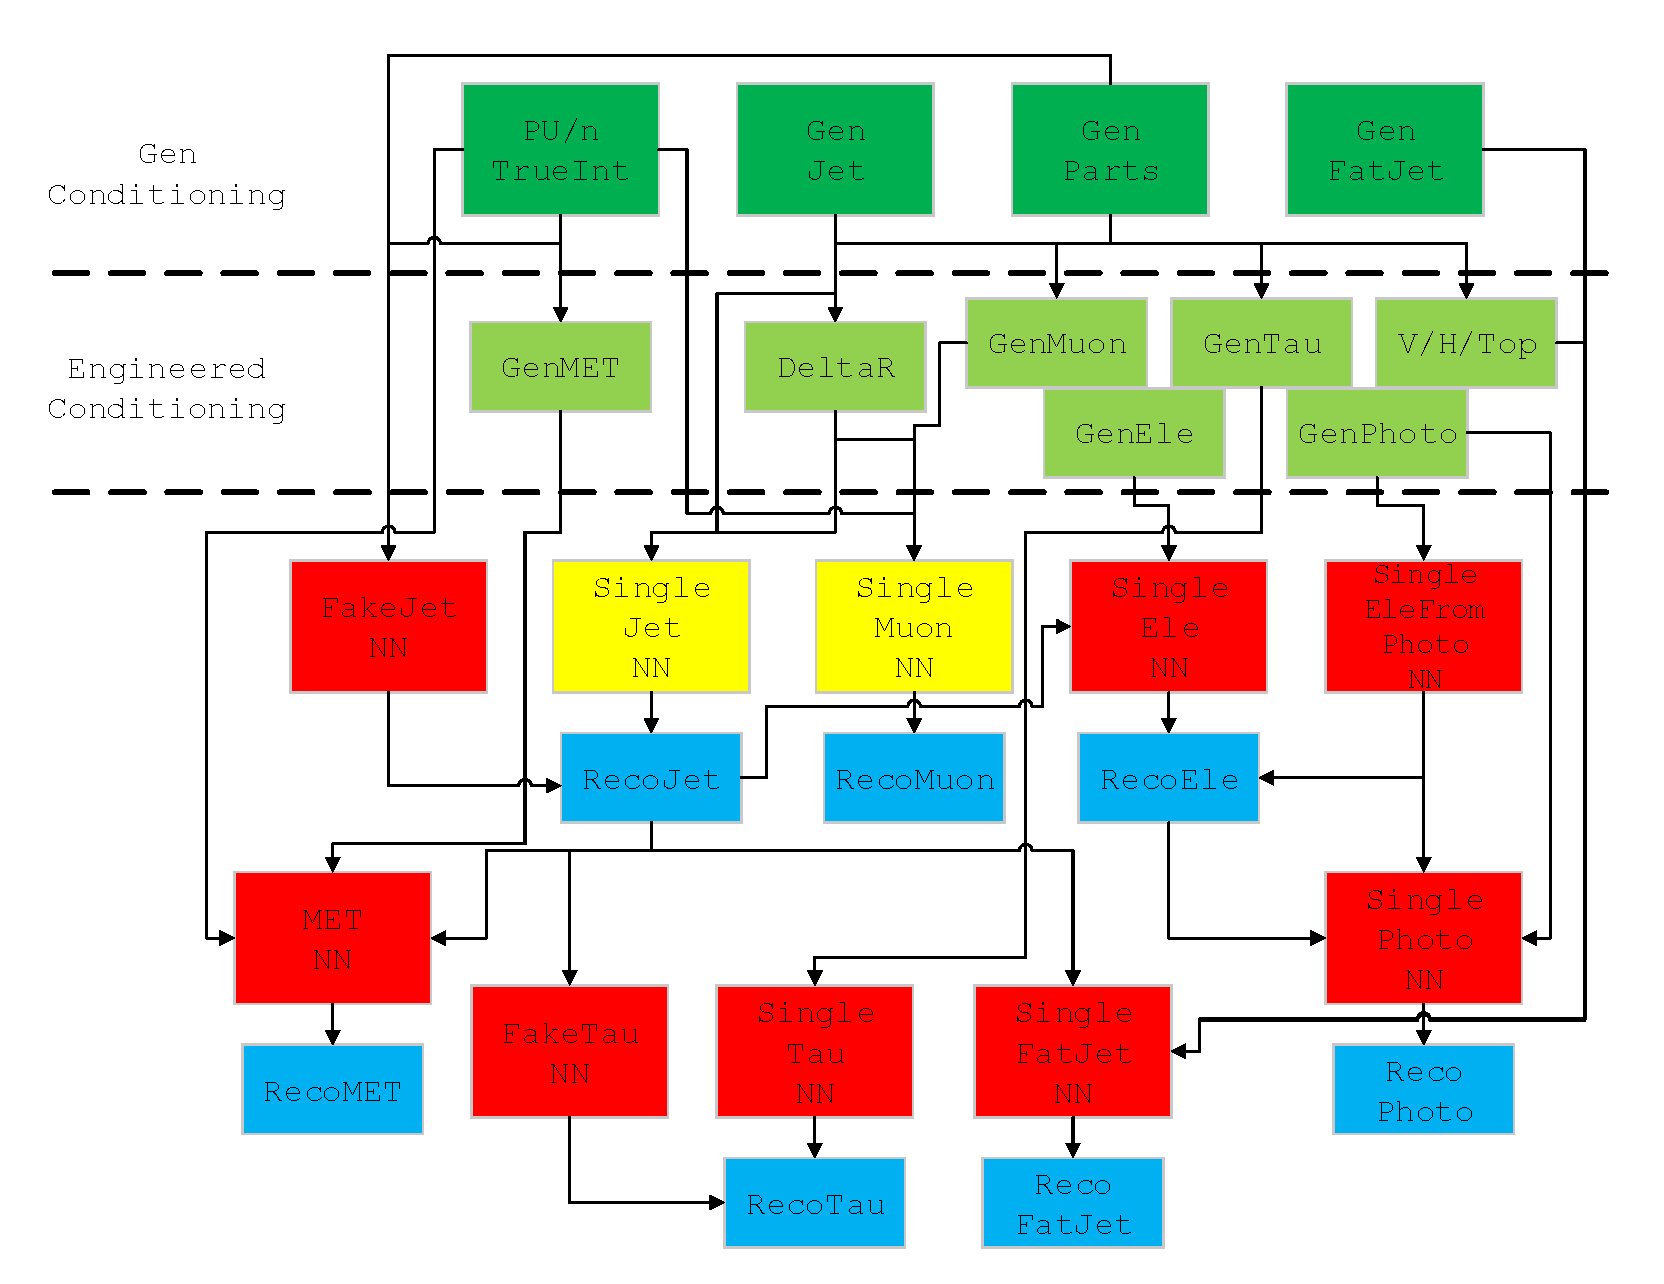
\includegraphics[width=\linewidth]{gfx/ch7/fullnanoaod.pdf}
    \caption[A global picture]{A possible global picture illustrating the various dependencies between conditioning, single object networks and RECO outputs.}
    \label{fig:globpic}
\end{figure}

\subsection{Optimization}
An important series of steps in the prototype end-to-end generator need to be optimized. 
First of all, the Gen-level quantities currently extracted from existing FullSim NanoAODs and written to file for processing could actually be produced from a dedicated FlashNano-Generator, capable of passing the desired inputs directly to our models without the need of previously existing files.

The ML models forming the backbone of our approach need to be properly optimized and thoroughly examined to find the best combination of hyperparameters, size and performance. Additionally, the training and the generation procedure may be modified to be run in parallel over multiple machines or clusters, providing significant speed adavantages. Another very serious issue to be addressed by the collaboration is the fact that our research is based on a series of \texttt{Python} packages maintained by a series of open-source contributors with no interest in the specific HEP use case and no assurance of continued and prolonged support, as well as backward compatibility.

The issue may be addressed in several ways. A possibility would be to experiment with splines-based models such as ours with the current packages, but once found the optimal transformation, the splines and their parameters could be mapped into a more convenient \texttt{C/C++} framework to be used and actively maintained by one of the computing groups of CERN, and possibly integrated as part of the \texttt{ROOT} language.

Additionally, the postoprocessing step needs to be revised with the addition of a check for numerical instabilities causing nonphysical values for the target distributions. These may be then easily corrected by regenerating the faulty event with another set of random noise as input.

\section{Future research}
The need for fast and reliable computing methods in the physical sciences, notably in the high-energy field, has fueled much of the technological progress of modern times. Despite this, the average physicist has generally little time to spend on innovating and improving its computing toolkit, and has to content himself with boilerplate solutions. This is especially true in highly specialized fields, such as HEP, which purse a wide variety of research directions.

Specifically, in recent years, ML techniques have been massively adopted by scientific collaborations around the world. However, such tools remain geared towards the necessities of industry; much work remains to be done to enable the use of this technologies in hard sciences.

As physicists with a keen interest in this type of applications, while still retaining useful domain knowledge, we are convinced that significant results could be achieved by pursuing the following research directions. 

\subsection{Other Flow-based applications in HEP}

The versatility of Normalizing Flows make them an optimal choice for tackling a wide range of problems, namely all those where the definition and manipulation of \emph{pdf}s is of vital importance.

We already mentioned a series of possible approaches in Section \ref{sec:nfapp}. The most interesting is possibly the approach to \emph{anomaly detection}, where Flows have already been used to define empirical distributions from data (see \cite{Kasieczka_2021}). Other interesting approaches being currently tested and deployed at CERN make use of ML approaches as unbiased function approximants for unknown, empirical pdfs (e.g. \cite{D_Agnolo_2019}), however, perhaps being generally less known, NF have yet to be tested as a solution to the problem.

\subsection{Graph Networks and Normalizing Flows}

Possibly considered the holy grail of ML for HEP applications at the LHC, the problem of \emph{track reconstruction} is mostly a pattern recognition task whose complexity grows much more than linearly with the increase of number of collisions, hence the number of tracks, and is thus expected to be one of the main problems for HL-LHC. When investigating such a large feature space, a common approach is to reduce the complexity of the network while still retaining useful information about local features through the use of \emph{Convolutional Neural Networks} (CNNs), which nowadays are the standard approach for image datasets (as pioneered in \cite{simonyan2015deep}).
Unfortunately, any representation of tracking detector as images
would look very sparse and would not benefit of the locality idea of the CNN. 

Another hard HEP problem is the reconstruction of secondary vertices used for b-tagging. In order to identify b-jets, a useful feature is the presence of the so called \emph{secondary vertices} in a jet, i.e. points in space, displaced from the interaction point, where a group of tracks
appears to originate from.

A promising way to overcome these challenges is the introduction of \emph{Graph Networks} (GNs), which represent input and output data as graphs to exploit any invariance of the graph itself in order to perform the dimensionality reduction that is achieved in CNN. In the case of a GN, the locality is not based on an euclidean metric like as before, but rather on the number of connections needed to reach one node from another. In order to enforce this kind of locality, a \emph{Message Passing} schema is often used for GN: the computation happens in several iterations where each iteration propagates information to/from neighbor nodes. Even a simple overview of the method goes beyond the scope of this section: we will now comment briefly on specific HEP advantages of this architecture, referring the reader to the seminal work of Battaglia \emph{et al.} \cite{battaglia2018relational} for a comprehensive review.

The key idea behind GNs in HEP is to represent the data as a graph where the nodes are the hits (i.e. the individual measurements from tracking sensors) and nodes of subsequent layers are connected (with some pruning of nonphysical connections). The output is instead a graph made of several disconnected branches each representing an
individual track (or track seed). We would like to emphasize how a \emph{graph input topology} would possibly benefit many other models already in use at LHC, allowing a better application simply by performing a preprocessing step through the use of GN layers. An interesting work in this direction, proposing a new approach that considers a jet as an unordered set of its constituent particles, effectively a "particle cloud" is the one presented by Qu and Gouskos \cite{pj2020}. Based on the particle cloud representation, they proposed ParticleNet, a customized neural network architecture using Dynamic Graph Convolutional Neural Network for jet tagging problems. The ParticleNet architecture achieves state-of-the-art performance on two representative jet tagging benchmarks and is improved significantly over existing methods. 

The graph topology may be extended to the Normalizing Flow approach as well. The autors of \cite{https://doi.org/10.48550/arxiv.2105.09016} introduced \emph{Equivariant Normalizing Flows} based on graph networks as the building block for defining equivariant invertible functions acting on graphs and capable of translating the NF approach to the generation of molecular structures.

In a similar vein, we could imagine to generate graph structures representing our target particle cloud representation, paving the way for an entirely new and powerful simulation approach at a completely different level from what discussed in the present work.

\subsection{Quantum Machine Learning}

Finally, a novel discipline born from \emph{Quantum Computing} and ML, known as \emph{Quantum Machine Learning} (QML) is already under serious investigation from the scientific community, due to the potential and significant \emph{quantum} advantages. The limits of what machines can learn have always been defined by the computer hardware we run our algorithms on—for example, the success of modern-day deep learning with neural networks is enabled by parallel GPU clusters.

Quantum machine learning extends the pool of hardware for machine learning by an entirely new type of computing device—the \emph{quantum computer}. Some research focuses on ideal, universal quantum computers (“fault-tolerant QPUs”) which are still years away. But there is rapidly-growing interest in quantum machine learning on near-term quantum devices (\emph{Noisy Intermediate-Scale Quantum} or NISQ).

We can understand these devices as special-purpose hardware like Application-Specific Integrated Circuits (ASICs) and Field-Programmable Gate Arrays (FPGAs), which are more limited in their functionality but nonetheless well suited to specific applications. In the modern viewpoint, quantum computers can be used and trained like neural networks. We can systematically adapt the physical control parameters, such as an electromagnetic field strength or a laser pulse frequency, to solve a problem. Additionally, quantum circuits are differentiable, and a quantum computer itself can compute the change in control parameters needed to become better at a given task. Trainable quantum circuits can be leveraged in other fields like quantum chemistry or quantum optimization. It can help in a variety of applications such as the design of quantum algorithms, the discovery of quantum error correction schemes, and the understanding of physical systems.

At the moment the effort of the HEP community is focused on quantum generative models (see \cite{chan2021quantum}), where the noisy behavior is mitigated or even beneficial. The CERN has already established a partnership with IBM, a leading competitor for quantum technologies, and founded the CERN Quantum Technology Initiative (CERN QTI), a comprehensive R$\&$D, academic and knowledge-sharing initiative to exploit quantum advantage for high-energy physics and beyond. 